\chapter{Introduction}

\section{The central dogma}

At the core of every living being is its genetic inheritance. The genetic
inheritance is what is being passed down from parents to their offspring, and
contains a blueprint detailing how to construct a new individual in a process
called \define{embryogenesis}. This genetic inheritance is physically present in
the form of \dna in every living cell\footnote{And to some extent in non-living
particles called \define{viruses}.}.

If the \dna is a library containing a blueprint of the cell’s instructions, then
there is need also for librarians, and for workers who enact the instructions
found in the blueprint and conveyed by the librarians. These find their
counterparts in living cells in the form of \mrna and \define{proteins}. The
process by which genetic information is stored in the \dna, conveyed by
\mrna[s], and enacted by proteins is formalised in the \emph{Central Dogma of
molecular biology}.

\begin{figure}[h!]
    \centering
    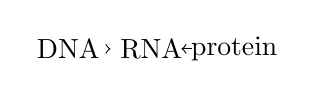
\begin{tikzpicture}
        [every node={circle, draw, inner sep=1em}, node distance=3em]
        \node (dna) {DNA};
        \node (rna) [right of=dna] {RNA};
        \node (protein) [right of=rna] {protein};
        \draw [->] (dna) -- (rna);
        \draw [->] (rna) -- (protein);
    \end{tikzpicture}
    \figcap{dogma}{The central dogma of molecular biology.}{}
\end{figure}

\todo[inline]{\begin{enumerate}[noitemsep,nolistsep,leftmargin=*]
    \item Molecular structure of DNA (bases, 5'--3', phosphoribose)
    \item DNA copying (strands, complementarity)
    \item Central dogma
    \item Template, coding strand, mRNA, proteins, genetic code
    \item Different polymerases, ncRNA
    \item DNA sequence as string
    \item Molecular and functional structure description of pol2 and pol3
\end{enumerate}}

\todo{Take intro from paper}

\subsection{Aside: modern modifications to the central dogma and evolution}

\subsection{Transcription}

\subsection{Posttranscriptional modification}

In particular A-to-I conversion (deamination), which is relevant in tRNA gene
wobble base pairing!

\subsection{Translation}

\subsection{The role of \abbr{trna}s in translation}

\section{Gene expression and its regulation}

\section{Using high-throughput sequencing for whole-genome analysis}

\subsection{Explain history and technology of \abbr{hts}}

\section{Types of non-coding \abbr{rna}, their function and expression}

\section{Structure of this thesis}
